

%----------------------------------------------------------------------------------------

\newpage

\section*{Synthesis of studied processes}{Synthèse des processus étudiés}




\bpar{
We conclude this introducing chapter by a synthesis and a perspective on interaction processes that have been identified in the theoretical and empirical analysis and in the literature. This will allow to situate the reviews of modeling entreprises to which we will proceed in chapter~\ref{ch:modelinginteractions}, and then will be compared to the one we will establish in the case of models.
}{
Nous concluons ce chapitre introductif par une synthèse et une mise en perspective des processus d'interaction identifiés par l'analyse théorique, empirique et la littérature. Celle-ci permettra de situer les revues des entreprises de modélisation auxquelles nous procéderons dans le chapitre~\ref{ch:modelinginteractions}, puis pourra être comparée à celle que nous établirons dans le cas des modèles.
}



\subsubsection*{A entry by scales}{Une entrée par les échelles}

\bpar{
A first entry to synthesize the processes considered consists in considering then by scale. We have seen that a multi-scale reading was relevant, and that it allowed globally to isolate characteristic spatial and temporal scales: microscopic, mesoscopic and macroscopic, with a rather good correspondence between temporal and spatial scales. This typology remains of course reduced, since it simplifies the class of processes that could result of these correspondences, for exemple a mobility at a large scale, or a bifurcation of the urban system which happens quickly, Similarly, processes that are themselves multi-scalar (the governance of Greater Paris is a good illustration, since it relates to governance levels and territorial issues at different scales) are taken into account in a simplified way. The axis complementary to the one of scales is based on ``effects and causes'': although we still remain within the frame of a complex causality as presented in introduction, we have unveiled processes for which it is possible to identify a precursor among the network or the territory (we will then denote them by $A \rightarrow B$), others are intrinsically complex and already contain circular causalities (for example in the case of governance processes), we will denote them by Networks $\leftrightarrow$ Territories. The synthesis table is then given in Table~\ref{tab:thematic:processes}.
}{
Une première entrée pour synthétiser les processus abordés consiste à les considérer par échelle. Nous avons vu qu'une lecture multi-échelle était pertinente, et que celle-ci permettait globalement de dégager des échelles spatiales et temporelles caractéristiques : microscopique, mesoscopique et macroscopique, avec une assez bonne correspondance des échelles spatiales et temporelles. Cette typologie est bien sûr réduite, puisqu'elle simplifie la classe des processus qui pourraient sortir de ces correspondances, par exemple une mobilité à grande échelle, ou une bifurcation du système urbain qui se manifeste rapidement. De même, les processus eux-mêmes multi-échelles (la gouvernance du Grand Paris en est une bonne illustration, mobilisant des niveaux de gouvernance et des enjeux territoriaux à différentes échelles) sont pris en compte de manière simplifiée. L'axe complémentaire à celui des échelles se base sur les ``effets et causes'' : bien que nous restions toujours dans le cadre d'une causalité complexe comme présenté en introduction, nous avons mis en évidence des processus pour lesquels il est possible d'identifier un précurseur parmi le réseau ou le territoire (nous les noterons alors $A \rightarrow B$), d'autres sont intrinsèquement complexes et contiennent déjà des causalités circulaires (par exemple dans le cas des processus de gouvernance), nous les noterons Réseaux $\leftrightarrow$ Territoires. Le tableau de synthèse est alors donné en Table~\ref{tab:thematic:processes}.
}


%%%%%%%%%%%%%
\begin{table}%[h!]
\caption[Interaction processes between networks and territories][Processus d'interaction entre réseaux et territoires]{\textbf{Interaction processes between networks and territories.} We synthesize the processes according to scales and the precursor typology.\label{tab:thematic:processes}}{\textbf{Processus d'interaction entre réseaux et territoires.} Nous synthétisons les processus selon les échelles et selon la typologie de sens.\label{tab:thematic:processes}}
\bpar{
\begin{tabular}{|l|p{5cm}|p{5cm}|p{5cm}|}
\hline
 & Networks $\rightarrow$ Territories & Territories $\rightarrow$ Networks & Networks $\leftrightarrow$ Territories\\ \hline
Micro & Mobility patterns & Network congestion ; Negative externalities & Mobility and social structure \\ \hline
Meso & Relocations ; Local effects of infrastructures & Potential breakdown & Metropolitan planning ; TOD \\ \hline
Macro & Interactions between cities ; Tunnel effect & Hierarchical differentiation of accessibility & Large scale planning ; Structural dynamics ; Bifurcations\\ \hline
\end{tabular}
}{
\begin{tabular}{|l|p{5cm}|p{5cm}|p{5cm}|}
\hline
 & Réseaux $\rightarrow$ Territoires & Territoires $\rightarrow$ Réseaux & Réseaux $\leftrightarrow$ Territoires\\ \hline
Micro & Motifs de mobilité & Congestion du réseau ; Externalités négatives & Mobilité et structure sociale \\ \hline
Meso & Relocalisations ; Effets locaux des infrastructures & Rupture de potentiel & Planification métropolitaine ; TOD \\ \hline
Macro & Interactions entre villes ; Effet tunnel & Différenciation hiérarchique de l'accessibilité & Planification à grande échelle ; Dynamique structurelle ; Bifurcations\\ \hline
\end{tabular}
}
\end{table}
%%%%%%%%%%%%%



\subsubsection*{A entry by actors}{Une entrée par les acteurs}

% imbrication hierarchique des concepts ? bof


\bpar{
A second entry privileges the role of \emph{actors}, i.e. of agents which make the territory. Indeed, the problematics linked to mobility concern the microscopic agents, the ones linked to accessibility urban and economic actors, the ones linked to planning governance actors. This aspect can be summarized by the scheme in Frame~\ref{frame:networkterritories:acteurs}.
}{
Une deuxième entrée privilégie le rôle des \emph{acteurs}, c'est-à-dire des agents qui font le territoire. En effet, les problématiques liées à la mobilité concernent les agents microscopiques, celles liées à l'accessibilité des acteurs urbains et économiques, celles liées à la planification des acteurs de gouvernance. Cet aspect peut être résumé par le schéma en Encadré~\ref{frame:networkterritories:acteurs}.
}


%%%%%%%%%%%%%
\begin{figure}[h!]
\begin{mdframed}
\bpar{
\includegraphics[width=\textwidth]{Figures/Theory/processes_acteurs_en}
}{
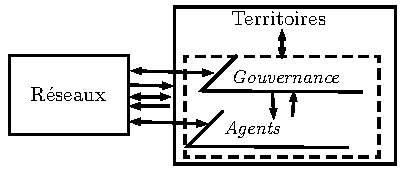
\includegraphics[width=\textwidth]{Figures/Theory/processes_acteurs}
}
\medskip
\framecaption{\textbf{An entry by actors on territorial systems.}\label{frame:networkterritories:acteurs}}{\textbf{Une entrée sur les systèmes territoriaux par les acteurs.}\label{frame:networkterritories:acteurs}}
\end{mdframed}
\end{figure}
%%%%%%%%%%%%%


\bpar{
In this scheme, we identify the territorial actors within the territorial system, which can be schematically formulated on two scales: agents at the microscopic scale which will be central for mobility processes, and governance actors at larger scales, which lead the governance processes. They interact between them in a complex way, and are here conceptually separated by dashed lines from others aspects of the territory to which thay are also strongly coupled.
}{
Dans ce schéma, on identifie les acteurs territoriaux au sein du système territorial, qui se déclinent schématiquement sur deux échelles : les agents à l'échelle microscopique qui seront centraux pour les processus de mobilité, et les acteurs de gouvernance à des échelles supérieures, qui mènent les processus de gouvernance. Ils interagissent entre eux de manière complexe, et sont séparés ici conceptuellement par les pointillés d'autres aspects du territoire avec lesquels ils sont aussi couplés fortement.
}


\bpar{
This entry can be put in perspective with the conceptual frame of~\cite{le2010approche}, which studies the links between the urban form and mobility practices within metropolitan contexts. This framework understands the urban system as a strong coupling between the location system, the activity system and the transportation system, by recalling the influence of demand agents (micro-economic agents) and planning agents (governance agents) on each system. The transportation system corresponds to our networks and the two other systems to an aspect of territorial agents, which also contain agents formulated within this frame. This parallel must be nuanced when changing scales: at the scale of the system of cities, when agents are cities, the location system has no meaning anymore, since it is adapted to a scale at most metropolitan, and specifically to corresponding ontologies.
}{
Cette entrée peut être mise en perspective avec le cadre conceptuel de~\cite{le2010approche}, qui étudie les liens entre forme urbaine et pratiques de mobilité dans des contextes métropolitains. Celui-ci comprend le système urbain comme un couplage fort entre système de localisation, système d'activités et système de transport, en précisant l'influence des agents demandeurs (agents micro-économiques) et des agents aménageurs (agents de gouvernance) sur chaque système. Le système de transport correspond à nos réseaux et les deux autres systèmes à un aspect des agents territoriaux, qui contiennent aussi les agents précisés dans ce cadre. Ce parallèle reste à nuancer lorsqu'on change d'échelle : à celle du système de villes, lorsque les agents sont les villes, le système de localisation n'a plus de sens, puisque celui-ci est adapté à une échelle au plus métropolitaine, et surtout aux ontologies correspondantes.
}


\bigskip

\bpar{
This double entry to read interaction processes between networks and territories will on the one hand condition the literature review of models done in chapter~\ref{ch:modelinginteractions}, and will on the other hand be completed and specified after it. 
}{
Cette double entrée de lecture des processus d'interaction entre réseaux et territoires conditionnera d'une part la revue de littérature des modèles faite en chapitre~\ref{ch:modelinginteractions}, et sera d'autre part complétée et précisée à l'issue de celui-ci.
}



\stars



%----------------------------------------------------------------------------------------

\newpage


\section*{Chapter Conclusion}{Conclusion du Chapitre}



\bpar{
Territories interact in a complex way with networks, in particular transportation networks, as shown by the numerous empirical examples or the theoretical constructions we reviewed. At different typical temporal scales (the day, the decade, and the century), correspond spatial scales (urban, metropolitan and system of cities), and also processes (mobility, accessibility and relocations, systemic structural effects and bifurcations). Concrete situations witness of local realities expressed with different nuances, and processes carrying these abstract processes with different roles and interactions between them.
}{
Les territoires interagissent de manière complexe avec les réseaux, en particulier ceux de transport, comme montré par les nombreux exemples empiriques ou les constructions théoriques passés en revue. À différentes échelles temporelles typiques (le jour, la décennie et le siècle), correspondent des échelles spatiales (urbaine, métropolitaine et système de villes), ainsi que des processus (mobilité, accessibilité et relocalisations, effets systémiques structurels et bifurcations). Les situations concrètes témoignent de réalités locales déclinés avec différentes nuances, et des processus portant ces processus abstraits avec différents rôles et interactions entre eux.
}


\bpar{
We have in a first section clarified this notion of interaction between transportation networks and territories by constructing a theoretical frame which allows to consider them as components of the territorial system in it entirety. We have then suggested an approach by co-evolution to take into account this complexity. In order to better identify these notions on concrete geographical examples, we have developed in~\ref{sec:casestudies} two metropolitan case study which are current issues, and underlined the certainties in terms of accessibility impact for major infrastructure projects which are systematically accompanied by an uncertainty in terms of the trajectory of the system on a longer term. Finally, we propose in~\ref{sec:qualitative} an excursion through fieldwork elements in China, Guangdong.
}{
Nous avons dans une première section clarifié cette notion d'interaction entre réseaux de transports et territoires en construisant un cadre théorique qui permet de les considérer comme des composantes du système territorial dans son ensemble. Nous avons alors suggéré une approche par la co-évolution pour tenir compte de cette complexité. Afin de mieux cerner ces notions sur des exemples géographiques concrets, nous avons développé en~\ref{sec:casestudies} deux cas d'étude métropolitain d'actualité, et souligné les certitudes en termes d'impact d'accessibilité pour des projets majeurs d'infrastructures qui s'accompagnent systématiquement d'incertitude en terme de trajectoire du système à plus long terme. Enfin, nous proposons en~\ref{sec:qualitative} une excursion par des éléments de terrain dans le Guangdong, Chine.
}


\bpar{
At this stage, having introduced the thematic object of study, we propose more particularly to focus on approaches implying modeling, making the choice of a fundamental role of the \emph{model} (on which we will come back with more details) in the production of knowledge.
}{
À ce stade, ayant introduit l'objet d'étude thématique, nous proposons de nous intéresser plus particulièrement aux approches impliquant une modélisation, faisant le choix d'un rôle fondamental du \emph{modèle} (sur lequel nous reviendrons plus en détails par la suite) dans la production de connaissance.
}



\stars


%-------------------------



